\شروع‌مسئله[24]
آرایه‌ای از اعداد داریم و می‌خواهیم آن را مرتب کنیم. در هر مرحله می‌توانیم یک زیرمجموعه از اندیس‌های آرایه انتخاب کنیم و آن عناصر را با حفظ ترتیب به ابتدای آرایه منتقل کنیم. به طور مثال اگر آرایه $\langle54,132,47,96\rangle$ باشد و اندیس‌های $1$ و $3$ را انتخاب کنیم، عناصر $54$ (که اندیس $1$ دارد) و $47$ که اندیس $3$ دارد با حفظ ترتیب به ابتدای آرایه می‌آیند و نتیجه می‌شود $\langle54,47,132,96\rangle$.
در پاسخ به موارد زیر اثبات دقیق ادعای خود را بیان کنید.
\شروع{زیرمسائل}
\زیرمسئله[12]
ثابت کنید برای مرتب‌سازی این آرایه در بدترین حالت، حداقل $\Omega(\log n)$ مرحله نیاز است.
\پاسخ{
	$P_n$ 
	را آرایه‌ای نزولی از 
	$n$
	  عضو در نظر میگیریم.
	
	لم: برای مرتب کردن 
	$P_n$
	 (به صورت صعودی) حداقل به
	  $\log n$
	   مرحله نیاز است.
	
	
	اثبات. 
	لم را به استقرا روی $n$ ثابت می کنم. 
	
	پایه: برای
	 $n=1$
	 صفر مرحله نیاز است.
	
	گام: فرض میکنم حکم به ازای
	 $n<k$
	  برقرار است. 
	
	$P_k$ 
	را در نظر بگیرید بعد از یک مرحله، یا حداقل
	 $\frac{k}{2}$
	  تا هستند که انتخاب نشده اند یا حداقل $\frac{k}{2}$ تا هستند که انتخاب شده اند این 
	  $\frac{k}{2}$
	   تا در هر دو صورت ترتیبشان نسبت به هم عوض نشده اگر در ادامه بقیه اعضا را درنظر نگیریم برای مرتب کردن این 
	   $\frac{k}{2}$
	    تا عضو طبق فرض استقرا به حداقل 
	    $\log \frac{k}{2}=\log k -1$
	     حرکت نیاز داریم که اگر حرکت اول را نیز حساب کنیم پس برای مرتب کردن $\frac{k}{2}$تا حداقل به
	      $\log k$
	       تا عملیات نیاز داریم.\\
}
\نمره‌دهی{
	آوردن مثالی که در آن حداقل به 
	$\Omega (\log n)$
	مرحله نیاز است ۴ نمره دارد (در بعضی راه‌حل‌ها برای این قسمت اثبات وجودی آوردند، آن‌ها هم نمره را گرفته‌اند).\\
	۸ نمره باقیمانده به اثبات تعلق گرفته.\\
}
\زیرمسئله[12]
الگوریتمی ارائه دهید که هر آرایه را در حداکثر
$O(\log n)$
مرحله مرتب کند. درستی الگوریتم خود را اثبات کنید.

\پاسخ{
	میانه اعداد را در نظر بگیرید و آن را $x$ بنامید، اعدادمان را به دو بخش کوچکتر مساوی $x$ و بیشتر از $x$ تقسیم می‌کنیم. سپس هر یک از این دو بخش را به صورت \textbf{همزمان} حل می‌کنیم، یعنی نهایتا در آرایه‌مان، اعداد کوچکتر از $x$، نسبت به یکدیگر مرتب شده‌اند و اعداد بزرگتر از $x$ نیز نسبت به یکدیگر مرتب شده‌اند. در گام آخر نهایتا اندیس‌های کوچکتر از $x$ را انتخاب کرده و آن‌ها را به ابتدای آرایه می‌آوریم.
	
	$$T(N) = T(\ceil{\frac{N}{2}}) + 1 \rightarrow T(N) \in \theta(\log{N})$$
}
\نمره‌دهی{
روش دیگر حل به کمک نمایش مبنای دو و استفاده از مرتب‌سازی مبنایی بود که آن نیز در صورت درستی، نمره کامل را کسب کرده است. راه‌‌حل‌های غلط نیز نمره‌ای تقریبا برابر با صفر گرفته‌اند.
}

\پایان{زیرمسائل}

\شروع‌مسئله[12] 
در بازی اسنِیک، یک جدول $n\times n$ داریم که یک مار تمام خانه‌های آن را مشابه شکل زیر پوشانده است و از یک خانه نیز دوبار عبور نکرده است.

\begin{center}
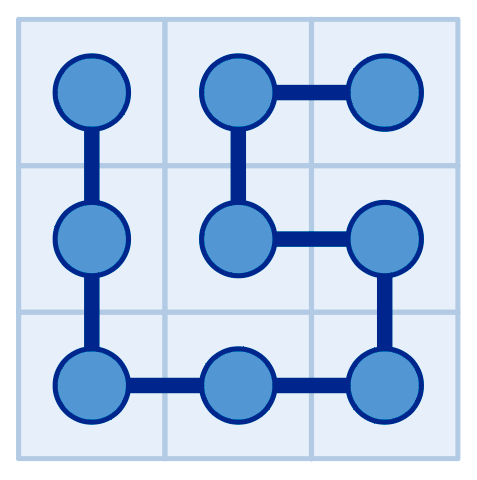
\includegraphics[width=0.3\columnwidth]{1c1d413eda7cf3fb3602564daddd634b1eb9b7e4.png}
\end{center}

شما در هر مرحله می‌توانید به طور دلخواه یک زیرجدول را انتخاب کنید و این سؤال را بپرسید که زوجیت تعداد بارهایی که مار مرز این جدول را قطع می‌کند چند بار است؟ به طور مثال در شکل زیر ما چهار بار مرز زیرجدول را رد می‌کند و جواب سؤال زوج است.

\begin{center}
	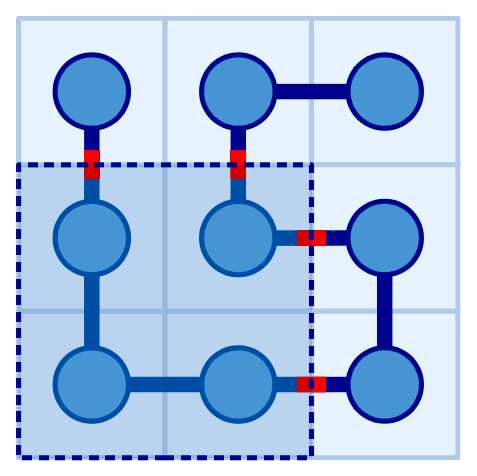
\includegraphics[width=0.3\columnwidth]{70064c8b6a8291d558472df2eb428c8bfbafd56c.png}
\end{center}

الگوریتمی طراحی کنید که با $O(n)$ پرسش سر و ته مار را پیدا کند.

\پاسخ{
ابتدا توجه کنید که جواب یک زیرجدول فرد است، اگر و تنها اگر دقیقا یکی از سر یا ته مار درون آن باشد؛ و زوج است، اگر و فقط اگر هر دو یا هیچکدام درون زیر جدول باشند.

اکنون، ابتدا هر سطر و هر ستون را به عنوان زیرجدول می‌پرسیم. اگر سر و ته مار در دو سطر مختلف باشند، آن دو سطر جواب فرد و بقیه جواب زوج می‌دهند و اگر در یک سطر باشند، همه سطرها جواب زوج می‌دهند. به طور مشابه برای ستون ها نیز همین اتفاق می‌افتد. چون سر و ته مار در دو خانه مختلف‌اند، میان سطرها یا ستون‌ها (یا هر دو) دو جواب فرد پیدا می‌شود. یعنی سر و ته مار در آن دو سطر (یا دو ستون) هستند.
حال کافیست تمام خانه‌های آن دو سطر (یا دو ستون) را تک تک بپرسیم تا سر و ته مار را پیدا کنیم.
زمان اجرای این الگوریتم 
$4 \times O(n) = O(n)$
 است.
	
}

\نمره‌دهی{	
برای بیان پاراگراف اول 3 نمره در نظر گرفته شده و اثبات دقیق آن الزامی نیست. اگر الگوریتم پیشنهاد شده درست باشد، نمره این بخش هم داده می‌شود. 
در مجموع، سختگیری زیادی نشده و به تمام الگوریتم‌های درست، نمره کامل داده شده ‌است و 
از راه‌حل‌های ناقص متناسب با مقدار ناقص بودن آن‌ها نمره کم شده‌ است.

}
